% created by Leon
% leon.l.zhu@gmail.com

%%%%%%%%%%%%%%%%%%%%%%%%%%%%%%%%%%%%%
% Document properties and packages
%%%%%%%%%%%%%%%%%%%%%%%%%%%%%%%%%%%%%
\documentclass[a4paper,8pt,final]{memoir}

% misc
\renewcommand{\familydefault}{bch}	% font
\pagestyle{empty}					% no pagenumbering
\setlength{\parindent}{0pt}			% no paragraph indentation


% required packages (add your own)
\usepackage{flowfram}										% column layout
\usepackage[top=2cm,left=0cm,right=1cm,bottom=2cm]{geometry}% margins
\usepackage{graphicx}										% figures
\usepackage{url}		   									% URLs
\usepackage[usenames,dvipsnames]{xcolor}					% color
\usepackage{multicol}										% columns env.
	\setlength{\multicolsep}{0pt}
\usepackage{paralist}										% compact lists
\usepackage{tikz}

\usepackage{multicol}                                       % multi columns

%%%%%%%%%%%%%%%%%%%%%%%%%%%%%%%%%%%%%
% Create column layout
%%%%%%%%%%%%%%%%%%%%%%%%%%%%%%%%%%%%%
% define length commands
\setlength{\vcolumnsep}{\baselineskip}
\setlength{\columnsep}{\vcolumnsep}

% frame setup (flowfram package)
% left frame
\newflowframe{0.2\textwidth}{\textheight}{0pt}{0pt}[left]
	\newlength{\LeftMainSep}
	\setlength{\LeftMainSep}{0.2\textwidth}
	\addtolength{\LeftMainSep}{1\columnsep}
 
% small static frame for the vertical line
\newstaticframe{1.5pt}{\textheight}{\LeftMainSep}{0pt}

% content of the static frame
\begin{staticcontents}{1}
\hfill
\tikz{%
	\draw[loosely dotted,color=RoyalBlue,line width=1.5pt,yshift=0]
	(0,0) -- (0,\textheight);}%
\hfill\mbox{}
\end{staticcontents}

% right frame
\addtolength{\LeftMainSep}{1.5pt}
\addtolength{\LeftMainSep}{1\columnsep}
\newflowframe{0.7\textwidth}{\textheight}{\LeftMainSep}{0pt}[main01]


%%%%%%%%%%%%%%%%%%%%%%%%%%%%%%%%%%%%%
% define macros (for convience)
%%%%%%%%%%%%%%%%%%%%%%%%%%%%%%%%%%%%%
\newcommand{\Sep}{\vspace{1.5em}}
\newcommand{\SmallSep}{\vspace{0.5em}}

\newenvironment{Highlights}
	{\ignorespaces\textbf{\color{RoyalBlue} Highlights}}
	{\Sep\ignorespacesafterend}
	
\newcommand{\CVSection}[1]
	{\Large\textbf{#1}\par
	\SmallSep\normalsize\normalfont}

\newcommand{\CVItem}[1]
	{\textbf{\color{RoyalBlue} #1}}

\newcommand\litem[1]{\item{\bfseries #1,\enspace}}

%%%%%%%%%%%%%%%%%%%%%%%%%%%%%%%%%%%%%
% Begin document
%%%%%%%%%%%%%%%%%%%%%%%%%%%%%%%%%%%%%
\begin{document}

% Left frame
%%%%%%%%%%%%%%%%%%%%
\begin{figure}
	\hfill
	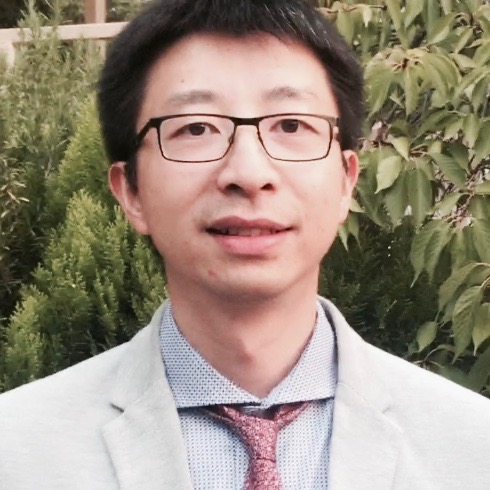
\includegraphics[width=0.6\columnwidth]{me}
	\vspace{-7cm}
\end{figure}

\begin{flushright}\small
\textbf{
	Liguang (Leon) Zhu \\
	\url{leon.l.zhu@gmail.com}  \\
%	\url{linkedin.com/in/liguangzhu/} \\
	+61 433 082 233}
\end{flushright}\normalsize
%
%\begin{flushright}\small
%	\CVSection{Skills}
%    \CVItem{Platforms}
%    \begin{multicols}{3}
%    \begin{compactitem}[\color{RoyalBlue}$\circ$]
%    	\item Lorem
%    	\item Ipsum
%    \end{compactitem}
%    \end{multicols}
%    \SmallSep

\framebreak


% Right frame
%%%%%%%%%%%%%%%%%%%%
\Huge\bfseries {\color{RoyalBlue} Liguang Zhu} \\
\Large\bfseries {\em Data Scientist} \\

\normalsize\normalfont

% About me
%\begin{Highlights}
%    \begin{itemize}
%        \item a
%        \item b
%        \item c
%    \end{itemize}
%% Lorem ipsum dolor sit amet, consectetur adipiscing elit. Vivamus vel bibendum metus. Proin rutrum pharetra molestie. Cras sollicitudin nulla nec leo lobortis in tristique purus pretium. Ut eu felis nulla. Pellentesque condimentum justo ut ligula feugiat nec facilisis tellus ultricies. Nullam sit amet dictum ipsum. Sed lacus neque, hendrerit eu rhoncus nec, pellentesque vitae sem.
%\end{Highlights}


% Highlights

\CVSection{Highlights}
    \begin{itemize}
        \item Strong skills in analytics and solution prototyping with R, Python and Weka.
%        \item Proven capablity of designing novel machine learning algorithms with probabilistic modeling and graph theory.
        \item Extensive experience in cross-disciplinary research, analytics and predictive modeling.
        \item Experienced in AWS, Microsoft Azure, high performance computing, and grid computing.
        \item Experienced in SQL, NoSQL, and data warehousing.
        \item Exposed to Hadoop and its ecosystem
    \end{itemize}
\Sep

% Experience
\CVSection{Experience}
\CVItem{Mar 2010 - Present, Clatyon School of IT, Monash University}\\
\underline{\textbf{Researcher \& PhD}}\\
\\
Specialise in data science disciplines including machine learning, probabilistic modeling, predictive modeling, and graph theory.
    \begin{itemize}
        \item Played a key role in researching and protyping of a novel feature engineering algorithm: Subsumption Resolution.
        \item Independently researched various predictive models on highly imbalanced biological data and implemented a tool for enzyme specificity prediction.
        \item Leading the design and development of a novel protein design pipeline by study high dimensional biological data.
        \item Designed one of the most stable protein molecules: FN3con.
        \item Designed a pharmaceutically promising molecule that challenges the current understanding of structure-folding relationship of proteins.
        \item Coordinated with research groups in different disciplines such as data science, structural biology, protein production unit, and chemical engineering.
    \end{itemize}
\Sep

\CVItem{Nov 2016 - Mar 2017, South East Water}\\
\underline{\textbf{Data Scientist Intern}}\\
\\
Responsible for exploring statistical and machine learning solutions to risk prediction and budget modeling of the gravity sewerage system.
    \begin{itemize}
        \item Utilised customer retention analysis for system failure modeling.
        \item Utilised customer segmentation analysis to reduce selection-bias.
        \item Explored and analysed datasets with various machine learning techniques such as classification, clustering, and association rule discovery.
        \item Sourced multiple datasets of CCTV inspections, historical renewal programs, and system failure records from data warehouses.
        \item Designed and implemented a budget optimisation software to maximise ROI.
        \item Utilised \textit{\textbf{Tableau}} for visual analytics and reporting.
    \end{itemize}
\Sep

\clearpage
\framebreak
\framebreak

\CVItem{Sep 2012 - Present, Monash University}\\
\underline{\textbf{Teaching Associate}}\\
\\
Responsible for delivering, facilitating, and managing tutorials, discussion, and practical laboratories.
    \begin{itemize}
        \item Advanced algorithms and data structures
        \item Business intelligence and data warehousing
        \item Introduction to data science
        \item Introduction to computer science
        \item programming foundations in Python
    \end{itemize}
\Sep

\CVItem{Sep 2010 - Dec 2010, School of Biological Science, Monash University}\\
\underline{\textbf{Research Assistant}}\\
\\
Responsible for the development and deployment of a portable database system on customised data collection devices for ecology research.
\Sep

\CVItem{Sep 2010 - Dec 2012, Fleet Software \& Services Pty Ltd}\\
\underline{\textbf{Freelancer Data Science Consultant}}\\
\\
Involved in the design and development of a value prediction system based on historical fleet exchange data.
    \begin{itemize}
        \item Managed data cleaning and predictive modeling.
        \item Minimised the average prediction error to \$600.
    \end{itemize}
\Sep
\Sep
\Sep
% Education
\CVSection{Education}
\CVItem{2012 - present, Monash University}\\
\underline{\textbf{Doctorate of Philosophy}}
\Sep

\CVItem{2008 - 2010, Monash University}\\
\underline{\textbf{Master of Computer Science (Minor Thesis in Data Science)}}
\Sep

\CVItem{2003 - 2007, Beijing Jiaotong University, China}\\
\underline{\textbf{Bachelor of Engineering in Computer Science with Honours}}
\Sep
\Sep
\Sep
% References

\CVSection{References}
Provide upon request.
%    \begin{multicols}{2}
%        %References upon request.
%        \textbf{Prof. Geoff Webb} \\
%        Director of Centre for Data Science \\
%        \textbf{Monash University} \\
%        +61 3 9905 3296 \\
%        \url{Geoff.Webb@monash.edu} \\
%
%        \textbf{Dr. Nayyar Zaidi} \\
%        Data Science Researcher \\
%        \textbf{Monash University} \\
%        +61 3 9905 3298 \\
%        \url{Nayyar.Zaidi@monash.edu} \\
%
%        \columnbreak
%
%        \textbf{Dr. Pramudi Suraweera} \\
%        Senior Data Scientist \\
%        \textbf{Seek.com} \\
%        +61 3 9905 3296 \\
%        \url{mailto: Geoff.Webb@monash.edu}
%    \end{multicols}
%\begin{ncolumn}{2}
% {\bf Prof Geoff Webb} & {\bf Dr Jiangning Song} \\
% Research professor & NHMRC Peter Doherty Fellow \\
% Faculty of IT, Monash University & Faculty of Medicine, Nursing and Health Sciences, Monash University \\
% Tel: +61 3 990 53296 & Tel: +61 3 990 29304 \\
% email: Geoff.Webb@monash.edu & email: Jiangning.Song@monash.edu \\


% {\bf Dr Pramudi Suraweera} & {\bf Dr Rohan Clarke} \\
% Data Analyst & Lecturer \\
% Deloitte Australia & Faculty of Science, Monash University \\
% Tel: +61 3 990 53219 & Tel: +61 3 990 51968 \\
% email: pramudi@gmail.com & email: Rohan.Clarke@monash.edu

%\begin{ncolumn}{2}
%{\bf Prof. Geoff Webb} 					&	{\bf Dr. Pramudi Suraweera}				\\
%Director of Centre for Data Science			&	Analytics Engagement Manager	 			\\
%{\bf  Monash University}			&  	Research, Insights \&  Analytics, {\bf Telstra}	\\
%p: +61 3 9905 3296 					& 	p: +61 3 8697 5439		\\
%e: Geoff.Webb@monash.edu 				& 	e: pramudi.suraweera@team.telstra.com		\\
%\\
%
%{\bf Dr. Pramudi Suraweera}
%Senior Data Scientist
%
%%{\bf Dr. Nayyar Zaidi} 					&	{\bf Dr. Arun S. Konagurthu}			\\
%%Data Science Researcher				&	Computational Biology Researcher	 				\\
%%{\bf  Monash University}	&  		{\bf  Monash University}		\\
%%p: +61 3 9905 3298 					& 	p: +61 3 9905 3227				\\
%%e: Nayyar.Zaidi@monash.edu				& 	e: Arun.Konagurthu@monash.edu		\\
%%\\
%
%{\bf Dr. Nayyar Zaidi} 					&	{\bf Mr. Duncan Sinclair}			\\
%Data Science Researcher				&	Team Leader Asset Management	 				\\
%{\bf  Monash University}	&  		{\bf  South East Water}		\\
%p: +61 3 9905 3298 					& 	p: +61 3 9552 3483				\\
%e: Nayyar.Zaidi@monash.edu				& 	e: Duncan.sinclair@sew.com.au		\\
%\end{ncolumn}


% Skills
%\CVSection{Skills}
%\CVItem{Platforms}
%\begin{multicols}{3}
%\begin{compactitem}[\color{RoyalBlue}$\circ$]
%	\item Lorem
%	\item Ipsum
%\end{compactitem}
%\end{multicols}
%\Sep
%
%\CVItem{Computer software}
%\begin{multicols}{3}
%\begin{compactitem}[\color{RoyalBlue}$\circ$]
%	\item Lorem
%	\item Ipsum
%	\item Dolor
%	\item Sit
%	\item Amet
%	\item Consectetur
%	\item Adipiscing
%	\item Elit
%	\item \ldots
%\end{compactitem}
%\end{multicols}
%\Sep

%\CVSection{Something other}
%aa
\clearpage
\framebreak
\framebreak

\CVSection{Publications}
\begin{itemize}
    \item B. Porebski, S. Keleher, J. Hollins, A. Nickson, \textbf{L. Zhu}, et. al. (2016) \textit{Smoothing a rugged protein folding landscape by sequence-based redesign.} Scientific Report, 6, Art. no. 33958.
    \item B.T. Porebski, A.A. Nickson, D.E. Hoke, M.R. Hunter, \textbf{L. Zhu}, S. McGowan, G.I. Webb, and A.M. Buckle. (2015). \textit{Structural and dynamic properties that govern the stability of an engineered fibronectin type III domain.} Protein Engineering, Design and Selection. 28(3): 67-78. Oxford University Press.
    \item \textbf{L. Zhu}, B.T. Porebski, A.M. Buckle, G.I. Webb. (2013). \textit{A probabilistic approach to In Silico protein design}. QMB E3: Enzyme Engineering and Evolution. Queenstown, New Zealand.
    \item B.T. Porebski, \textbf{L. Zhu}, D.E. Hoke, W. Dai, S. Keleher, N.A. Borg, S.P. Bottomley, G.I.Webb, A.M. Buckle. (2013). \textit{A structural, biophysical and computational investigation of two sequence-based protein engineering methods}. Poster session presented at: The 38th Lorne Conference on Protein Structure and Function. Lorne, Victoria.
    \item F. Zheng, G.I. Webb, P. Suraweera, and \textbf{L. Zhu}. (2012). \textit{Subsumption Resolution: An Efficient and Effective Technique for Semi-Naive Bayesian Learning.} Machine Learning 87(1): 93-125. Springer Netherlands.
\end{itemize}
\Sep


%%%%%%%%%%%%%%%%%%%%%%%%%%%%%%%%%%%%%
% End document
%%%%%%%%%%%%%%%%%%%%%%%%%%%%%%%%%%%%%
\end{document}
